\section{Durchführung und Aufbau}
\label{sec:Durchführung}
Ziel des Versuches ist es sich mit de Grundlagen der Vakuumtechnik vertraut zu machen und das Saugvermögen sowie die Leckrate von einer Drehschiebepumpe als auch einer Trubopumpe zu bestimmen. Eine Skizze des Aufbaus ist in Abbildung \ref{??} zu sehen. 
\begin{figure}[htpb]
  \centering
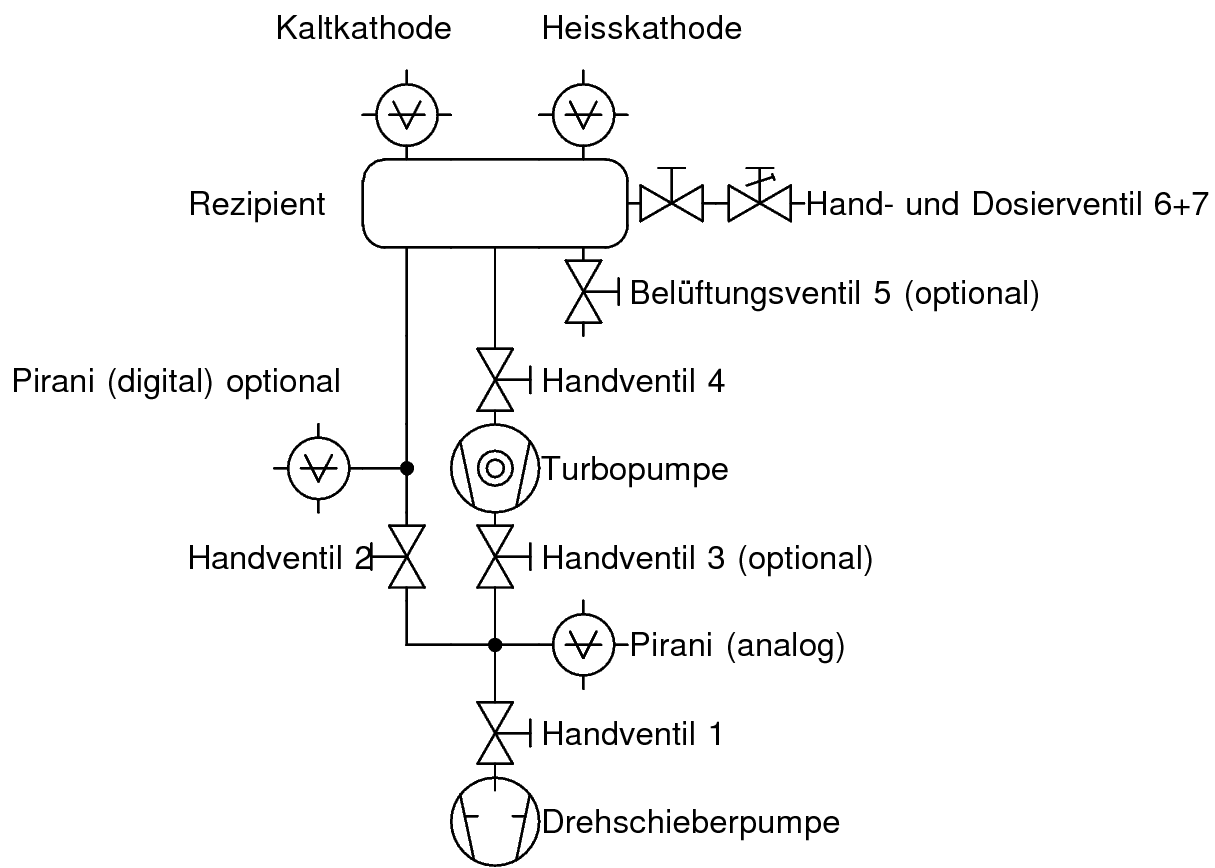
\includegraphics[width=0.8\textwidth]{picture/pumpaufbau.png}
\caption{Schema des Aufbaus des Pumpstandes \cite{Pfeiffer}}
  \label{fig:pump}
\end{figure}
Beim Aufbau des Vakuumstandes wurde darauf geachtet das Volumen des System möglichst gering zu halten um das System übersichtlich zu halten. Alle Dichtungen sind Handfest zugezogen und der Rezipient erwärmt worden um das Ausgasen zu verrringern. \newline
Zunächst soll die p(t)-Kurve aufgenommen werde. Dafür wurde der Pumpstand wie in Abbildung \ref{fig:Dreh} zu sehen aufgebaut. 
\begin{figure}[htpb]
  \centering
  \includegraphics[width=\textwidth]{picture/Aufbau1.png}
  \caption{Pumpstand zur Bestimmung der Kennziffern der Drehschieberpumpe}
  \label{fig:Dreh}
\end{figure}
Als erstes wird dafür der Maximaldruck der Drehschieberpumpe gemessen. Dazu muss das Überdruckventil (3 \& 4) geschlossen werden und der Druck durch die analoge Anzeige des Pirani-Messgerät(7) abgelse werden. Anschließend wird für 4 verschiedene Drücke jeweils zu 18 verschiedenen Drücken die Zeit genommen welche die Pumpe benötigt um diese zu errreichen. Die Messreihe wird jeweils 3-mal durchgeführt. 
Anschließend wird die Leckrate bestimmt indem das Überdruckventil so justiert wird, dass zwischen Saugvermögen und Luftsstrom ein Gleichgewichts von (0.1, 0.4, 0.8 und 1.0) eingestellt. Anschließend wird die Pume abgeklemmt und der Druck gegen die Zeit aufgenommen. Dies wird für jeden Gleichgewichtsdruck 5 mal wiederholt.  \newline
Um für die Turbopumpe ein hinreichend großes Vorvakuum zu produzieren muss der Aufbau modifiziert werde. Dazu wird der Luftstrom durch die Pumpepumpe, so wie es in Abbildung \ref{fig:??} zu sehen ist, geleitet
\begin{figure}[htpb]
  \centering
  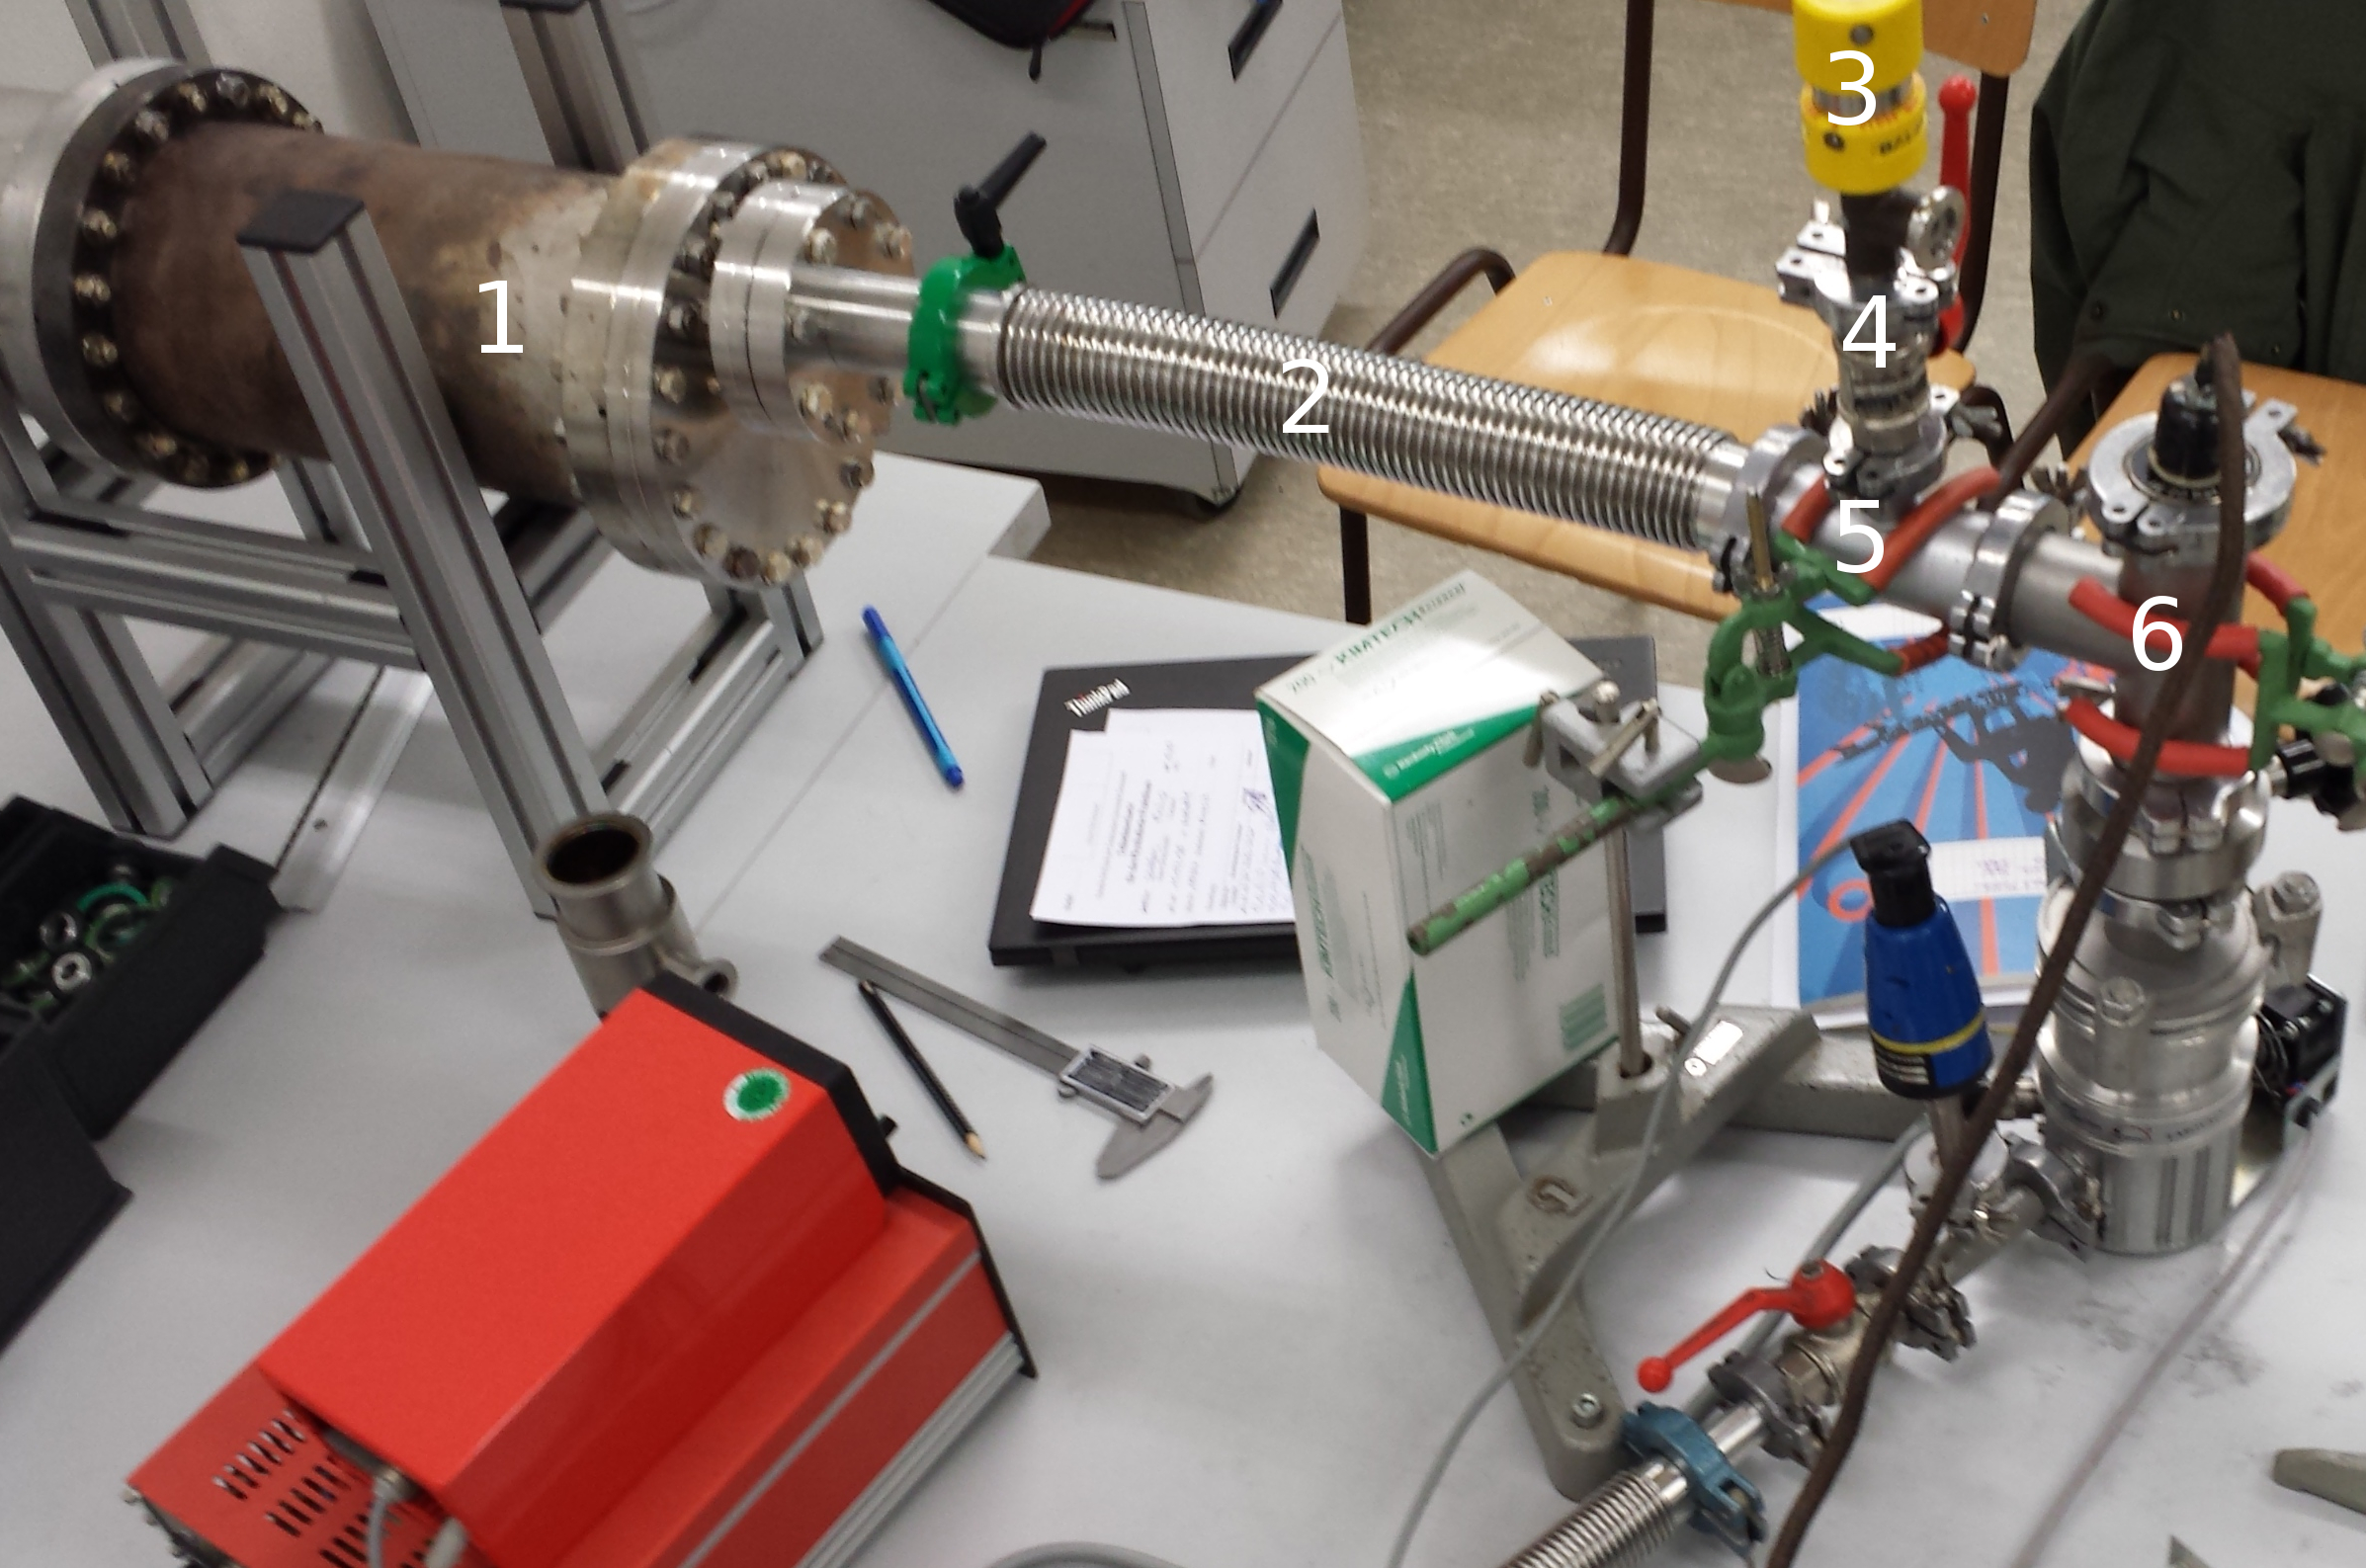
\includegraphics[width=\textwidth]{picture/Aufgabe2.png}
  \caption{<+caption text+>}
  \label{fig:<+label+>}
\end{figure}
Anschließend wird die selbe Messreihe wie bei der Drehschiebepumpe aufgenommen,  jedoch mit modifizierten Drücken. Es sollen 4 Leckratenmessreihen mit Startdrücken von 5bis $20*10^{-5}$ mbar durchgeführt werden und die p(t)-Messung jeweils von einem Druck von $5*10^{-3}$ mbar jeweils 3 Messungen. 
Zuletzt werden die Maße der Verwendeteten Objekte genommen um das Volumen des Evakuierten Raums zu schätzen. Darauf wird der Feher geschätzt weil die Innendurchmesser nicht immer mit den Messinstrumenten errreichbar sind.
